% Figure 1 -- Cognition-on-Engine (CoE) framework
% Two-tier diagram:
%   (top)    concrete walk-through: 3-colourings of a hexagon under Z_6
%   (bottom) abstract LLM <-> Domain Engine framework with R / T / C streams
% Compile:  pdflatex fig1_coe_framework_v2.tex
\documentclass[tikz,border=10pt]{standalone}
\usepackage{amsmath,amssymb}
\usepackage{xcolor}
\usepackage{tikz}
\usetikzlibrary{
    arrows.meta,
    positioning,
    calc,
    shapes.geometric,
    shapes.misc,
    backgrounds,
    fit,
}

% ---------- palette (cool, Nature-ish) ------------------------------------
\definecolor{cNavy}   {HTML}{08306B}
\definecolor{cBlue}   {HTML}{1F5FA8}
\definecolor{cBlueBg} {HTML}{E8F1FB}
\definecolor{cTeal}   {HTML}{2C7E7B}
\definecolor{cGreen}  {HTML}{41AE76}
\definecolor{cTealBg} {HTML}{E6F4F1}
\definecolor{cVio}    {HTML}{6A51A3}
\definecolor{cVioBg}  {HTML}{ECE7F2}
\definecolor{cAmber}  {HTML}{D08714}
\definecolor{cAmberBg}{HTML}{FBF1DD}
\definecolor{cInk}    {HTML}{222222}
\definecolor{cMute}   {HTML}{555555}
\definecolor{cFaint}  {HTML}{BBBBBB}

% Hexagon vertex colours: c=(0,1,2,0,1,2) -> R G B R G B
\definecolor{vR}{HTML}{D62728}
\definecolor{vG}{HTML}{2CA02C}
\definecolor{vB}{HTML}{1F77B4}

% ---------- styles --------------------------------------------------------
\tikzset{
    every node/.style={font=\small},
    boxbase/.style={
        rectangle, rounded corners=4pt,
        line width=0.8pt,
        inner sep=5pt,
        align=center,
    },
    qbox/.style    ={boxbase, draw=cBlue!70,  fill=cBlueBg, text width=2.7cm,
                     font=\footnotesize\linespread{1.05}\selectfont},
    constrbox/.style={boxbase, draw=cTeal!70, fill=cTealBg, text width=2.7cm,
                     font=\footnotesize\linespread{1.05}\selectfont},
    llmbox/.style  ={boxbase, draw=cNavy!80,  fill=cBlueBg, text width=3cm,
                     font=\footnotesize\linespread{1.05}\selectfont},
    outbox/.style  ={rectangle, rounded corners=3pt,
                     draw=cAmber!80, line width=0.7pt,
                     fill=cAmberBg, inner sep=4pt,
                     align=left,
                     font=\scriptsize\ttfamily\linespread{1.0}\selectfont},
    flow/.style    ={-{Latex[length=2.6mm,width=2.2mm]},
                     line width=0.9pt, color=cMute},
    rflow/.style   ={flow, draw=cBlue!85,  line width=1.1pt},
    tflow/.style   ={flow, draw=cGreen!85, line width=1.1pt},
    cflow/.style   ={flow, draw=cVio!85,   line width=1.1pt},
    qflow/.style   ={-{Latex[length=2.4mm,width=2mm]},
                     line width=0.9pt, dashed, draw=cMute},
    sectiontitle/.style={font=\bfseries, color=cInk},
    caption/.style={font=\scriptsize\itshape, color=cMute},
    smallcap/.style={font=\scriptsize, color=cMute},
}

\begin{document}
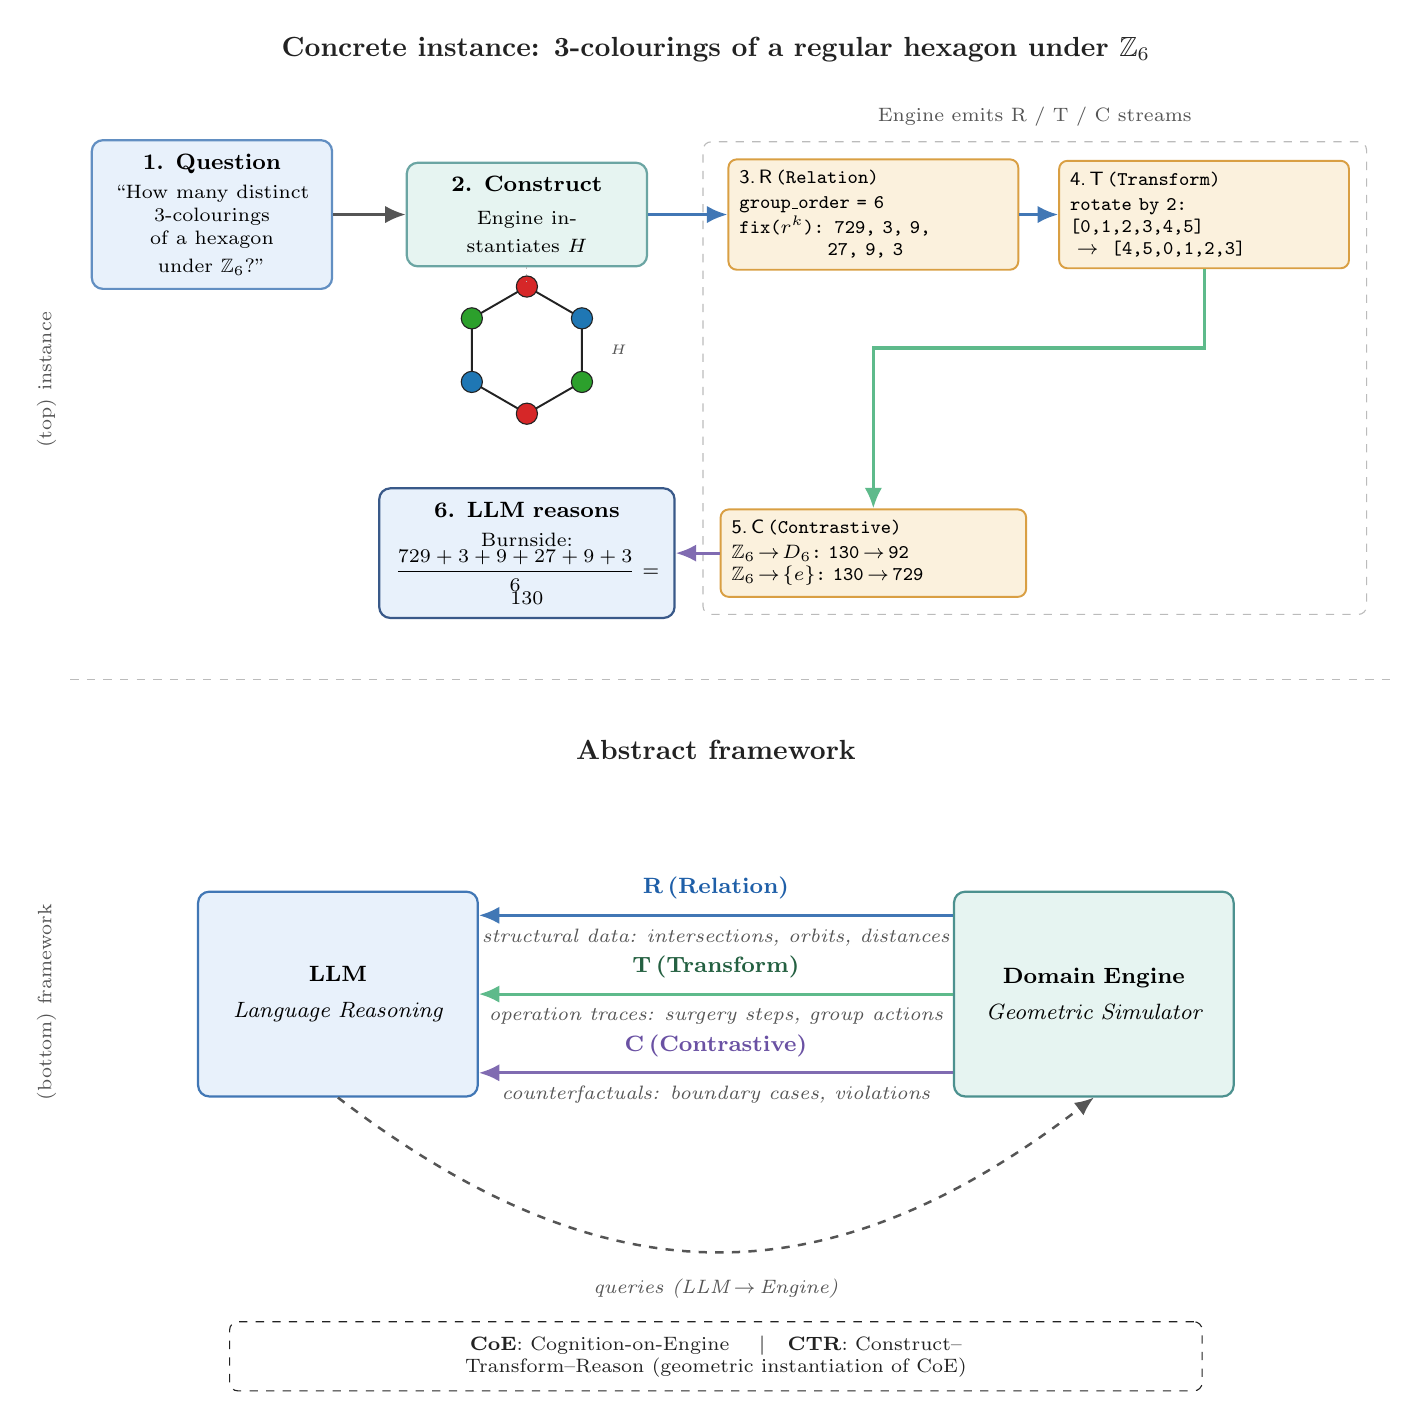
\begin{tikzpicture}[x=1cm, y=1cm]

% =========================================================================
%   T O P   T I E R  --  concrete walk-through
% =========================================================================

% Title (raised to leave a clear vertical gap above the bracket label)
\node[sectiontitle] at (8, 9.6)
    {Concrete instance: 3-colourings of a regular hexagon under $\mathbb{Z}_6$};

% --- Row 1: s1 --> s2 --> s3 --> s4  (left to right) ----------------------
\node[qbox, anchor=center] (s1) at (1.6, 7.5)
    {\textbf{1. Question}\\[2pt]
     \scriptsize ``How many distinct\\ 3-colourings of a hexagon\\ under $\mathbb{Z}_6$?''};

\node[constrbox, anchor=center] (s2) at (5.6, 7.5)
    {\textbf{2. Construct}\\[2pt]
     \scriptsize Engine instantiates~$H$};

\node[outbox, anchor=center, text width=3.4cm] (s3) at (10.0, 7.5)
    {\textbf{\normalfont\sffamily 3.\,R}\,(Relation)\\[1pt]
     group\_order = 6\\
     fix($r^k$): 729, 3, 9,\\
     \phantom{fix($r^k$):\,}27, 9, 3};

\node[outbox, anchor=center, text width=3.4cm] (s4) at (14.2, 7.5)
    {\textbf{\normalfont\sffamily 4.\,T}\,(Transform)\\[1pt]
     rotate by 2:\\
     {[0,1,2,3,4,5]}\\
     $\;\to\;$ {[4,5,0,1,2,3]}};

% --- Hexagon picture, tight under s2 (bigger: scale 0.85, all 6 verts) ---
\begin{scope}[shift={($(s2.south)+(0,-1.05)$)}, scale=0.85]
    % vertices at 90, 150, 210, 270, 330, 30 degrees
    \foreach \i in {0,...,5} {
        \coordinate (v\i) at ({90+60*\i}:0.95);
    }
    \draw[line width=0.7pt, color=cInk]
        (v0)--(v1)--(v2)--(v3)--(v4)--(v5)--cycle;
    % colours c = (R,G,B,R,G,B) -> v0,v1,v2,v3,v4,v5
    \foreach \i/\c in {0/vR, 1/vG, 2/vB, 3/vR, 4/vG, 5/vB} {
        \fill[\c] (v\i) circle (4.5pt);
        \draw[line width=0.4pt, color=cInk] (v\i) circle (4.5pt);
    }
    % tiny "H" annotation
    \node[font=\tiny\itshape, color=cMute, anchor=west]
          at ({0:1.1}) {$H$};
\end{scope}
% subtle dotted tether from s2 box bottom to hexagon top
\draw[color=cFaint, line width=0.4pt, dotted]
      (s2.south) -- ($(s2.south)+(0,-0.18)$);

% --- Row 2: s4 turns down --> s5 --> s6  (right to left) ----------------
\node[outbox, anchor=center, text width=3.6cm] (s5) at (10.0, 3.2)
    {\textbf{\normalfont\sffamily 5.\,C}\,(Contrastive)\\[1pt]
     $\mathbb{Z}_6\!\to\! D_6$:\ 130\,$\to$\,92\\
     $\mathbb{Z}_6\!\to\!\{e\}$:\ 130\,$\to$\,729};

\node[llmbox, anchor=center, text width=3.4cm] (s6) at (5.6, 3.2)
    {\textbf{6. LLM reasons}\\[2pt]
     \scriptsize Burnside:\\[1pt]
     $\dfrac{729+3+9+27+9+3}{6}=130$};

% Connectors: 1->2->3->4 in row 1, then 4 |- 5, then 5 -> 6 in row 2
\draw[flow]  (s1.east)  -- (s2.west);
\draw[rflow] (s2.east)  -- (s3.west);
\draw[rflow] (s3.east)  -- (s4.west);
% s4 turns DOWN then LEFT to s5 (clear right-angle, no diagonals)
\draw[tflow] (s4.south) -- ++(0,-1.0) -| (s5.north);
\draw[cflow] (s5.west)  -- (s6.east);

% Dashed bracket around the three R/T/C engine outputs (s3, s4, s5)
\begin{scope}[on background layer]
\node[draw=cFaint, line width=0.4pt, dashed,
      rounded corners=3pt, fit=(s3)(s4)(s5),
      inner sep=6pt] (rtcgroup) {};
\end{scope}
% Label centred directly above the bracket (rtcgroup.north is top-centre by
% construction). Small yshift just clears the dashed border.
\node[smallcap, anchor=south, align=center]
     at ($(rtcgroup.north)+(0,0.06)$)
     {Engine emits R / T / C streams};

% =========================================================================
%   D I V I D E R
% =========================================================================
\draw[color=cFaint, line width=0.4pt, dashed]
      (-0.2, 1.6) -- (16.6, 1.6);

% =========================================================================
%   B O T T O M   T I E R  --  abstract framework
% =========================================================================

\node[sectiontitle, anchor=center] at (8, 0.7)
    {Abstract framework};

% LLM and Engine boxes
\node[qbox, anchor=center, text width=3.2cm, minimum height=2.6cm,
      draw=cBlue!85, fill=cBlueBg] (LLM) at (3.2, -2.4)
      {\textbf{LLM}\\[3pt]\itshape\footnotesize Language Reasoning};

\node[constrbox, anchor=center, text width=3.2cm, minimum height=2.6cm,
      draw=cTeal!85, fill=cTealBg] (ENG) at (12.8, -2.4)
      {\textbf{Domain Engine}\\[3pt]\itshape\footnotesize Geometric Simulator};

% R stream (top of box)
\draw[rflow] ($(ENG.west)+(0,1.0)$) -- ($(LLM.east)+(0,1.0)$)
    node[midway, above=2pt, font=\footnotesize\bfseries, color=cBlue]
        {R\,(Relation)}
    node[midway, below=1pt, caption]
        {structural data: intersections, orbits, distances};

% T stream (middle)
\draw[tflow] ($(ENG.west)+(0,0.0)$) -- ($(LLM.east)+(0,0.0)$)
    node[midway, above=2pt, font=\footnotesize\bfseries, color=cGreen!55!black]
        {T\,(Transform)}
    node[midway, below=1pt, caption]
        {operation traces: surgery steps, group actions};

% C stream (lower portion of box, leaves room for queries arc below)
\draw[cflow] ($(ENG.west)+(0,-1.0)$) -- ($(LLM.east)+(0,-1.0)$)
    node[midway, above=2pt, font=\footnotesize\bfseries, color=cVio]
        {C\,(Contrastive)}
    node[midway, below=1pt, caption]
        {counterfactuals: boundary cases, violations};

% Feedback arrow: starts at LLM south-mid, big bow, ends at ENG south-mid.
% Bow drops well below the C stream (which is at y = -3.4) -- bottom of arc
% reaches y ~ -6.0, leaving > 2 cm of vertical separation from C.
\draw[qflow] (LLM.south) .. controls
    ($(LLM.south)+( 3.4,-2.6)$) and
    ($(ENG.south)+(-3.4,-2.6)$) ..
    (ENG.south);
\node[caption, anchor=north] at (8, -5.9)
      {queries  (LLM\,$\to$\,Engine)};

% Bottom caption strip
\node[draw=cFaint, line width=0.4pt, dashed,
      rounded corners=3pt, inner sep=5pt,
      text width=12cm, align=center,
      font=\scriptsize, color=cInk]
      at (8, -7.0)
      {\textbf{CoE}: Cognition-on-Engine
       \quad$\mid$\quad
       \textbf{CTR}: Construct--Transform--Reason
       (geometric instantiation of CoE)};

% Tier labels in left margin
\node[smallcap, rotate=90, anchor=center] at (-0.5, 5.4)
      {(top) instance};
\node[smallcap, rotate=90, anchor=center] at (-0.5, -2.5)
      {(bottom) framework};

\end{tikzpicture}
\end{document}
